\documentclass[11pt,a4paper]{article}
\usepackage[T1]{fontenc}
\usepackage[margin=1in]{geometry}
\usepackage{graphicx}
\usepackage{booktabs}
\usepackage{array}
\usepackage{hyperref}
\usepackage{placeins}
\hypersetup{hidelinks}

\title{Supplementary Material: TCVM-Net}
\author{Induj Gupta, Harthik Manichandra Vanumu, and Shrijani Patil\\
Manipal Institute of Technology Bengaluru,\\
Manipal Academy of Higher Education, Manipal, India\\
\texttt{induj.mitblr2023@learner.manipal.edu}\\
\texttt{harthik.mitblr2023@learner.manipal.edu}\\
\texttt{shrijani.mitblr2023@learner.manipal.edu}}
\date{}

\begin{document}
\maketitle

\section{Scope}
This supplementary material supports the paper ``TCVM-Net: Temporal Consistency Verification for Robust Traffic Surveillance Against Physical Adversarial Attacks''. It reports additional visual and reproducibility details derived from the same generated outputs used in the main manuscript. No additional manually estimated metrics are introduced.

\section{Contribution and Positioning Details}
Table~\ref{tab:supp_contrib} gives the claim boundary used for the compressed main paper.

\begin{table}[ht]
\centering
\small
\caption{Contribution-to-evidence map.}
\label{tab:supp_contrib}
\begin{tabular}{p{0.25\linewidth}p{0.34\linewidth}p{0.31\linewidth}}
\toprule
Contribution & Evidence & Boundary \\
\midrule
Temporal consistency defense & Track histories, confidence EMA, motion IoU, feature cosine score, disappearance recovery & Detects temporal inconsistency; does not certify robustness \\
Physical-style benchmark & Patch, sticker, reflective, motion blur, occlusion, and low-light attack splits with ASR logs & Software simulation; printed validation remains future work \\
Baseline comparison & YOLOv8n, YOLOv8s, image-only preprocessing, and AdvAug-YOLOv8n & AdvAug is matched-family robustness \\
Deployment analysis & FPS, latency, p95 latency, and memory on RTX 4060 Laptop GPU & Python TCVM has measurable latency overhead \\
\bottomrule
\end{tabular}
\end{table}
\FloatBarrier

\section{TCVM Inference Pseudocode}
\begin{enumerate}
    \item Run YOLOv8 on frame $I_t$ to obtain detections $\mathcal{D}_t$.
    \item Associate detections with active tracks using the tracker.
    \item For each tracked object, compute confidence, motion, feature, and disappearance consistency scores.
    \item Combine scores into the temporal anomaly score $A^k(t)$ and apply the detector-collapse gate to missing-track events.
    \item Accept stable detections; reject or recover short-gap predictions when $A^k(t)$ exceeds the threshold.
    \item Update histories conservatively so recovered detections do not poison the temporal prior.
\end{enumerate}

\section{Extended Attack Visualizations}
Figure~\ref{fig:supp_attack_gallery} shows representative physical-style perturbations used by the attack pipeline. The main paper uses these examples to illustrate perturbation families rather than to claim physical-world validation.

\begin{figure}[ht]
\centering
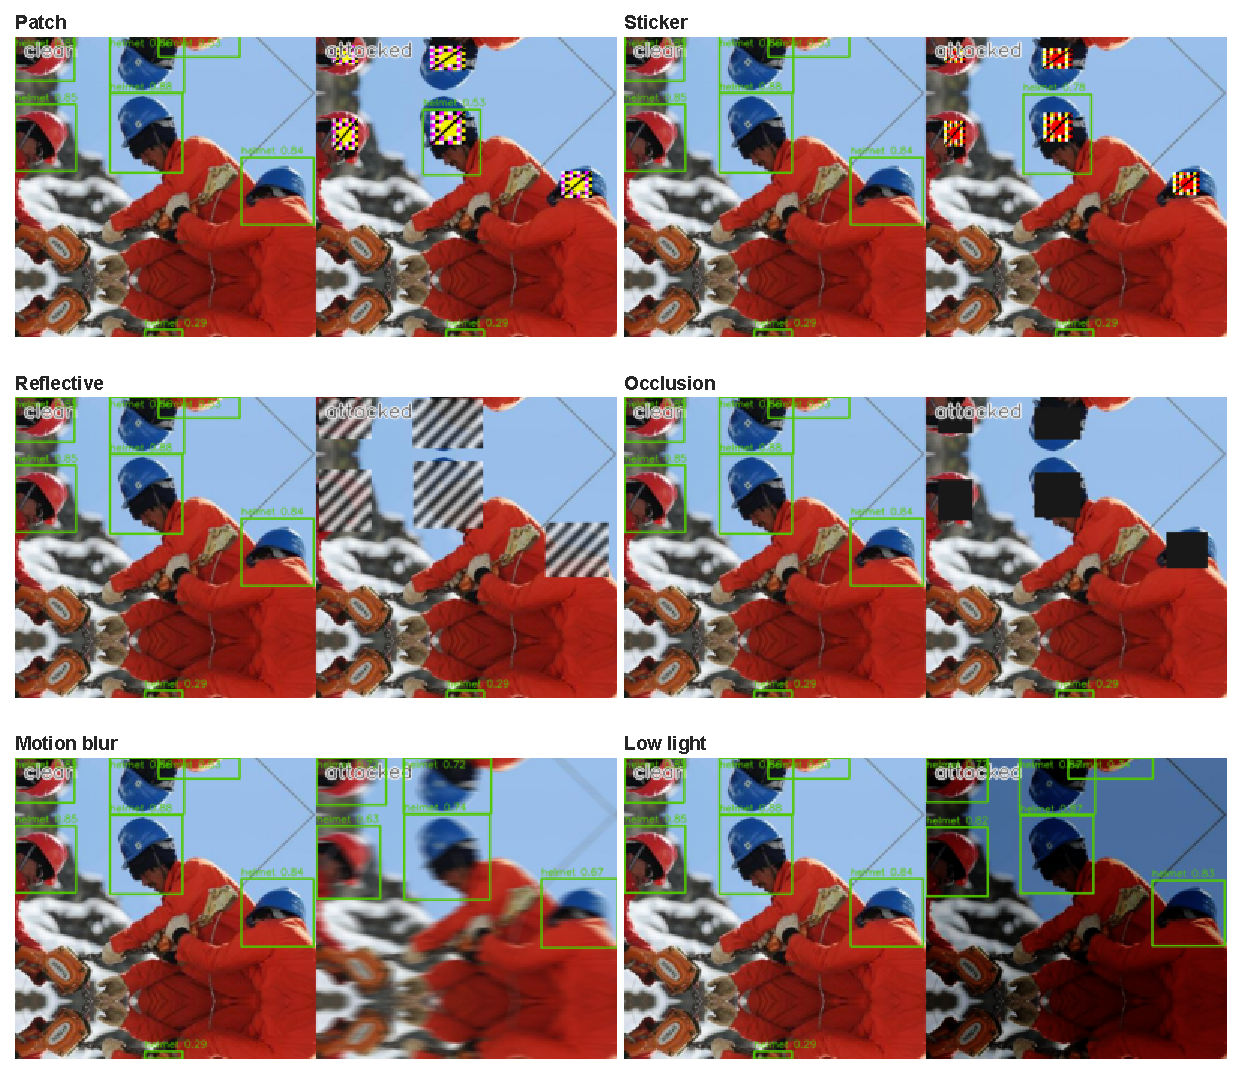
\includegraphics[width=\linewidth]{../outputs/figures/attack_gallery.pdf}
\caption{Representative patch, sticker, reflective, occlusion, motion-blur, and low-light attack panels.}
\label{fig:supp_attack_gallery}
\end{figure}
\FloatBarrier

\section{Attack Success-Rate Uncertainty}
Table~\ref{tab:attack_ci_auto} reports image-level bootstrap confidence intervals for attack success rate on the same 50-image held-out subset used in the main robustness table. The intervals are computed directly from per-image attack logs with 10,000 bootstrap resamples and fixed seed 2026.

\input{../paper/tables/attack_ci_auto.tex}
\FloatBarrier

\section{Additional Main-Paper Plots}
\begin{figure}[ht]
\centering
\includegraphics[width=0.85\linewidth]{../outputs/figures/robustness_comparison.pdf}
\caption{Attack-wise mAP@50 comparison for YOLOv8 and image-only preprocessing.}
\label{fig:supp_robustness}
\end{figure}

\begin{figure}[ht]
\centering
\includegraphics[width=0.85\linewidth]{../outputs/figures/advtrain_comparison.pdf}
\caption{Matched synthetic-family adversarial-augmentation comparison.}
\label{fig:supp_advtrain}
\end{figure}

\begin{figure}[ht]
\centering
\includegraphics[width=0.78\linewidth]{../outputs/figures/ablation_chart.pdf}
\caption{Ablation chart corresponding to the main-paper ablation table.}
\label{fig:supp_ablation}
\end{figure}

\begin{figure}[ht]
\centering
\includegraphics[width=0.72\linewidth]{../outputs/figures/fps_robustness_tradeoff.pdf}
\caption{Speed--robustness trade-off on the reflective temporal probe.}
\label{fig:supp_fps}
\end{figure}
\FloatBarrier

\section{Temporal Confidence and Anomaly Trajectories}
Figures~\ref{fig:supp_temporal_probe} and~\ref{fig:supp_temporal_video} show detector confidence and TCVM anomaly trajectories for the controlled reflective probe and the real-video pseudo-label stress test.

\begin{figure}[ht]
\centering
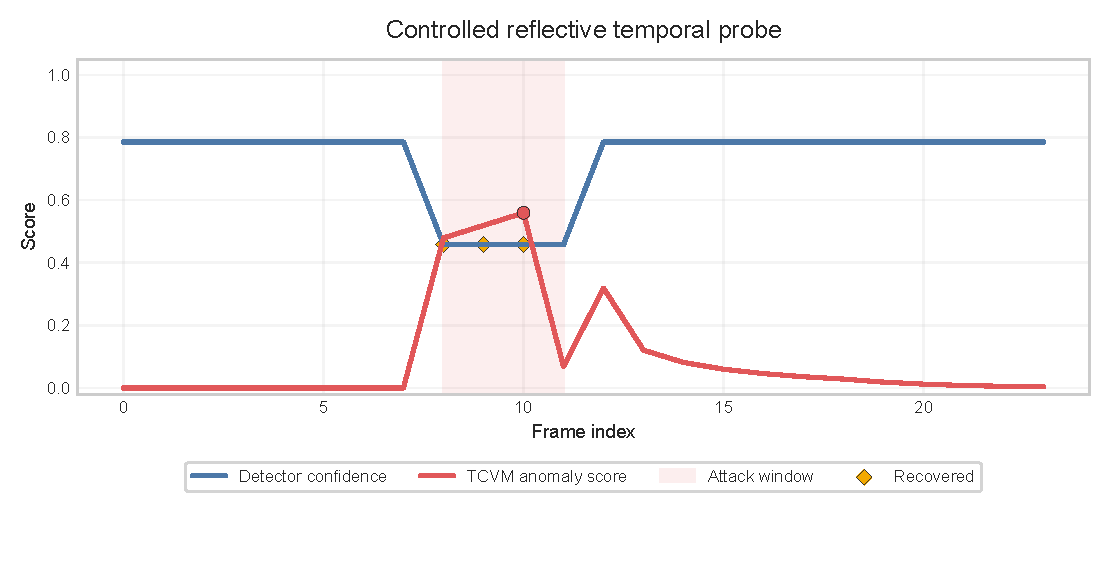
\includegraphics[width=0.92\linewidth]{../outputs/figures/temporal_confidence_reflective_probe.pdf}
\caption{Controlled reflective probe confidence and anomaly trajectory.}
\label{fig:supp_temporal_probe}
\end{figure}

\begin{figure}[ht]
\centering
\includegraphics[width=0.92\linewidth]{../outputs/figures/temporal_confidence_real_video_reflective.pdf}
\caption{Real-video reflective stress-test confidence and anomaly trajectory.}
\label{fig:supp_temporal_video}
\end{figure}
\FloatBarrier

\section{Annotated Public HELMET Pilot}
To reduce dependence on pseudo-label-only video evidence, we ran a small public-data pilot using the Kaggle HELMET dataset listed in the main bibliography. The pilot downloads 24 frames from the test clip \texttt{Bago\_highway\_10}, converts the provided motorcycle bounding boxes to YOLO labels, and applies full-box occlusion to annotated motorcycle boxes in source frames 52--54. This is an annotated public-video short-gap stress test, not a printed physical attack.

\input{../paper/tables/public_helmet_pilot_auto.tex}

\begin{figure}[ht]
\centering
\includegraphics[width=\linewidth]{../outputs/figures/public_helmet_pilot_gallery.pdf}
\caption{Clean and occluded frames from the public HELMET pilot. The sequence uses real traffic frames and human annotations; the occlusion overlay is software generated.}
\label{fig:supp_public_pilot_gallery}
\end{figure}

\begin{figure}[ht]
\centering
\includegraphics[width=0.92\linewidth]{../outputs/figures/temporal_confidence_public_helmet_pilot.pdf}
\caption{Temporal confidence and anomaly trajectory for the public HELMET short-gap occlusion pilot. The detector-count collapse gate promotes missing-track events during the attack interval and avoids most normal tracking gaps.}
\label{fig:supp_public_pilot_temporal}
\end{figure}

We also executed an expanded 20-clip public HELMET stress test using held-out clips listed in the generated metadata. The benchmark contains 480 real traffic frames and 4068 human motorcycle boxes. The perturbation is still synthetic, but the frames, scene motion, and annotations are public and video-based.

\input{../paper/tables/public_helmet_multiclip20_auto.tex}

The main ablation uses the same expanded public-video setting. It is included here with threshold sensitivity and runtime-mode tables so that reviewers can separate anomaly quality, threshold calibration, and deployment overhead. The scaled-flow rows quantify the strongest measured speed--sensitivity compromise: they preserve more anomaly F1 than the no-flow mode while substantially reducing dense optical-flow cost.

\input{../paper/tables/ablation_auto.tex}

\input{../paper/tables/tcvm_threshold_sensitivity_public_helmet_multiclip20_auto.tex}

\input{../paper/tables/tcvm_speed_modes_auto.tex}

\input{../paper/tables/tcvm_overhead_profile_public_helmet10_auto.tex}

\begin{figure}[ht]
\centering
\includegraphics[width=\linewidth]{../outputs/figures/public_helmet_multiclip10_gallery.pdf}
\caption{Clean and occluded frames from the 10-clip public HELMET benchmark. Only annotated attack-window frames receive the synthetic occlusion.}
\label{fig:supp_public_multiclip_gallery}
\end{figure}

\begin{figure}[ht]
\centering
\includegraphics[width=0.92\linewidth]{../outputs/figures/temporal_confidence_public_helmet_multiclip10.pdf}
\caption{Temporal confidence and anomaly trajectory for the 10-clip public HELMET benchmark. Vertical separators mark clip boundaries; shaded regions mark the repeated three-frame attack windows.}
\label{fig:supp_public_multiclip_temporal}
\end{figure}

\begin{figure}[ht]
\centering
\includegraphics[width=0.92\linewidth]{../outputs/figures/temporal_confidence_public_helmet_multiclip20.pdf}
\caption{Temporal confidence and anomaly trajectory for the expanded 20-clip public HELMET benchmark.}
\label{fig:supp_public_multiclip20_temporal}
\end{figure}

\begin{figure}[ht]
\centering
\includegraphics[width=0.84\linewidth]{../outputs/figures/tcvm_threshold_sensitivity_public_helmet_multiclip20.pdf}
\caption{Threshold sensitivity on the expanded 20-clip public HELMET benchmark. The chosen $\theta=0.45$ balances high attack-window recall with substantially lower false positives.}
\label{fig:supp_public_multiclip20_threshold}
\end{figure}

A separate 80-frame reflective HELMET stress case was also executed. It reduced COCO YOLOv8n motorcycle mAP@50 from 0.698 to 0.501, but TCVM-Net did not recover the sequence at the helmet-calibrated threshold. We keep this negative result as evidence that long reflective attacks and cross-task calibration remain unresolved.
\FloatBarrier

\section{Detector-Specific YOLOv8 Patch Pilot}
To address the concern that hand-designed sticker and reflective overlays may be weaker than detector-aware attacks, we optimized a printability-constrained EOT patch directly against YOLOv8 motorcycle confidence. The patch was optimized on eight public HELMET frames and evaluated on all 120 frames of the five-clip benchmark as a digital overlay. It is not claimed as printed physical validation. Running TCVM-Net on the patched sequence gives low anomaly recall, which is reported as a failure case for temporally persistent detector-specific attacks.

\input{../paper/tables/yolov8_patch_public_auto.tex}

\begin{figure}[ht]
\centering
\includegraphics[width=\linewidth]{../outputs/figures/public_helmet_yolov8_patch_gallery.pdf}
\caption{Detector-specific YOLOv8 patch overlay examples on public HELMET frames.}
\label{fig:supp_yolov8_patch_gallery}
\end{figure}
\FloatBarrier

\section{Grad-CAM Explanation}
\begin{figure}[ht]
\centering
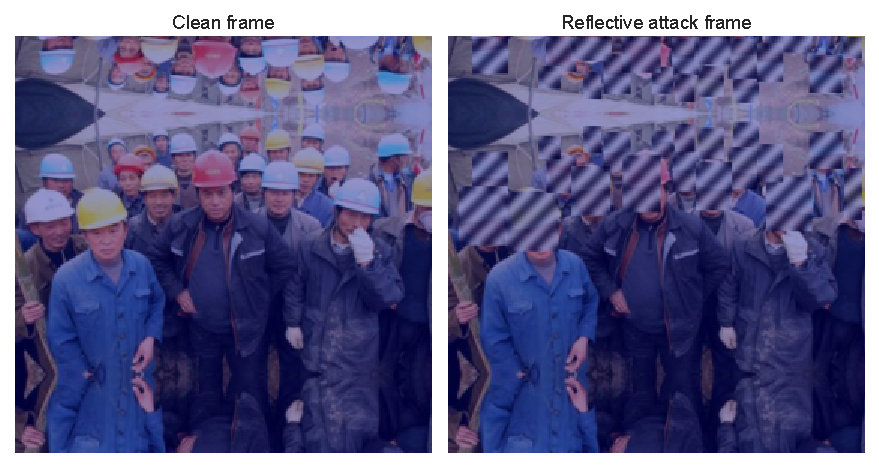
\includegraphics[width=0.85\linewidth]{../outputs/figures/gradcam_reflective_probe/gradcam_comparison.pdf}
\caption{Grad-CAM comparison before and during the reflective temporal attack.}
\label{fig:supp_gradcam}
\end{figure}
\FloatBarrier

\section{Threshold Sensitivity}
The real-video pseudo-label stress test evaluates TCVM-Net at thresholds 0.30, 0.45, and 0.62. The main finding is that lower thresholds increase attack-window recall but over-flag normal frames, while higher thresholds reduce false positives but may miss the attack interval. This motivates per-camera calibration before deployment.

\section{Hardware Benchmark Details}
The edge benchmark was executed on a Windows laptop with an NVIDIA GeForce RTX 4060 Laptop GPU using CUDA-enabled PyTorch. The measured dense-probe throughput was 8.49 FPS for YOLOv8 and 3.98 FPS for YOLOv8+TCVM-Net. Peak resident memory increased from 1102 MB to 1120 MB. On the public HELMET 10-clip profiling benchmark, quarter-resolution optical flow reached 13.48 FPS with 0.522 anomaly F1, while disabling flow reached 32.21 FPS with 0.420 anomaly F1. On the expanded 20-clip benchmark, full-resolution dense optical flow exhausted OpenCV memory, while quarter-flow completed at 18.14 FPS with 0.591 anomaly F1.

\section{Reproducibility Notes}
All paper tables are regenerated from CSV or JSON artifacts using the repository table-update script. Publication checks are executed with the publication-output validator, which verifies required result tables and figures.

\section{Physical Validation Protocol}
A low-cost printed-perturbation protocol is provided in the repository documentation. It is intended as an immediate follow-up experiment and is not used to add unexecuted metrics to the main paper.

\end{document}
